\item A viga fina, tendo massa de \SI{75}{\kilogram}, é suportada por dois cabos. Se o cabo na extremidade $B$ é cortado, de modo que a viga seja liberada do repouso quando $\theta=\SI{30}{^{\circ}}$, determine a velocidade com que a extremidade $A$ atinge a parede. Despreze o atrito em $B$.

\import{../answers}{answer-10}

\vspace{-1cm}
\begin{flushright}
	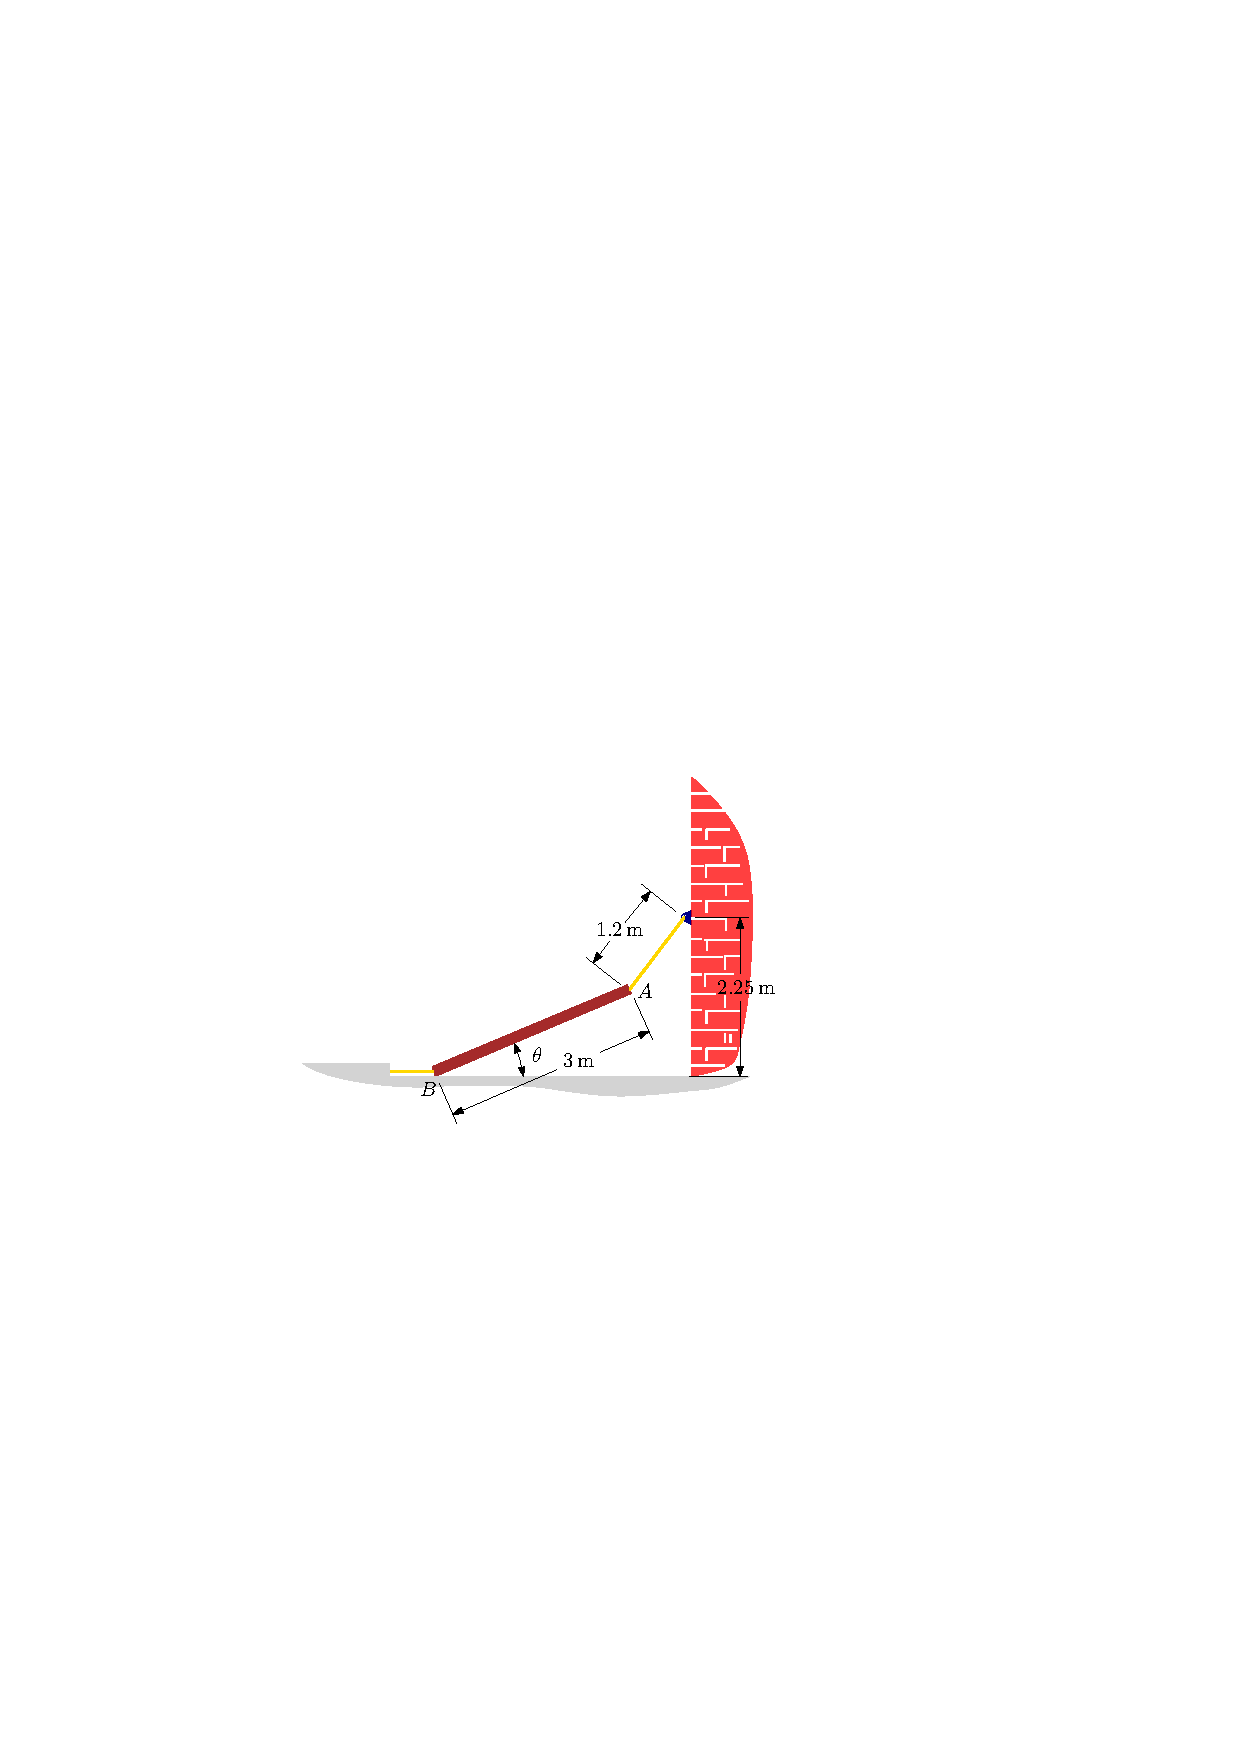
\includegraphics[scale=1.2]{../../images/draw_4_1}
\end{flushright}